\chapter{Simulation et analyse}
\label{chap:simulation}

\section{Introduction}

Ce chapitre exploite l'infrastructure sécurisée mise en place au chapitre précédent pour valider sa résilience face à des scénarios d'attaque réalistes. Il présente d'abord la simulation de la flotte IoT à partir d'un dataset multi-classes (76\,000 événements rejoués par 50 dispositifs Python), puis l'analyse réseau passive réalisée par Suricata avec ses règles personnalisées MQTT, et enfin l'agrégation et la corrélation des alertes dans le SIEM Wazuh. L'objectif est de démontrer la chaîne complète : génération de trafic mTLS $\to$ détection IDS $\to$ visualisation centralisée.

\section{Simulation de la flotte IoT}

\subsection{Présentation du dataset}

Le dataset utilisé est le \textbf{IoT Communication Security Dataset}, composé de 76\,000 entrées représentant des échanges MQTT typiques d'un écosystème IoT industriel. Chaque entrée décrit les caractéristiques d'une communication : protocole, longueur du payload, durée, type d'attaque éventuel.

\begin{table}[H]
\centering
\caption{Distribution des classes dans le dataset}
\label{tab:dataset_classes}
\begin{tabular}{lrl}
\toprule
\textbf{Classe} & \textbf{Occurrences} & \textbf{Description} \\
\midrule
Normal & 43\,200 & Trafic IoT légitime \\
DoS & 12\,600 & Inondation de connexions/messages \\
MiTM & 8\,400 & Interception et modification de paquets \\
Replay & 5\,600 & Rejeu de messages capturés \\
FalsifiedData & 3\,900 & Injection de données falsifiées \\
Scanning & 1\,400 & Scan de ports et d'infrastructure \\
Malware & 840 & Comportements de type botnet \\
\bottomrule
\end{tabular}
\end{table}

\begin{figure}[H]
  \centering
  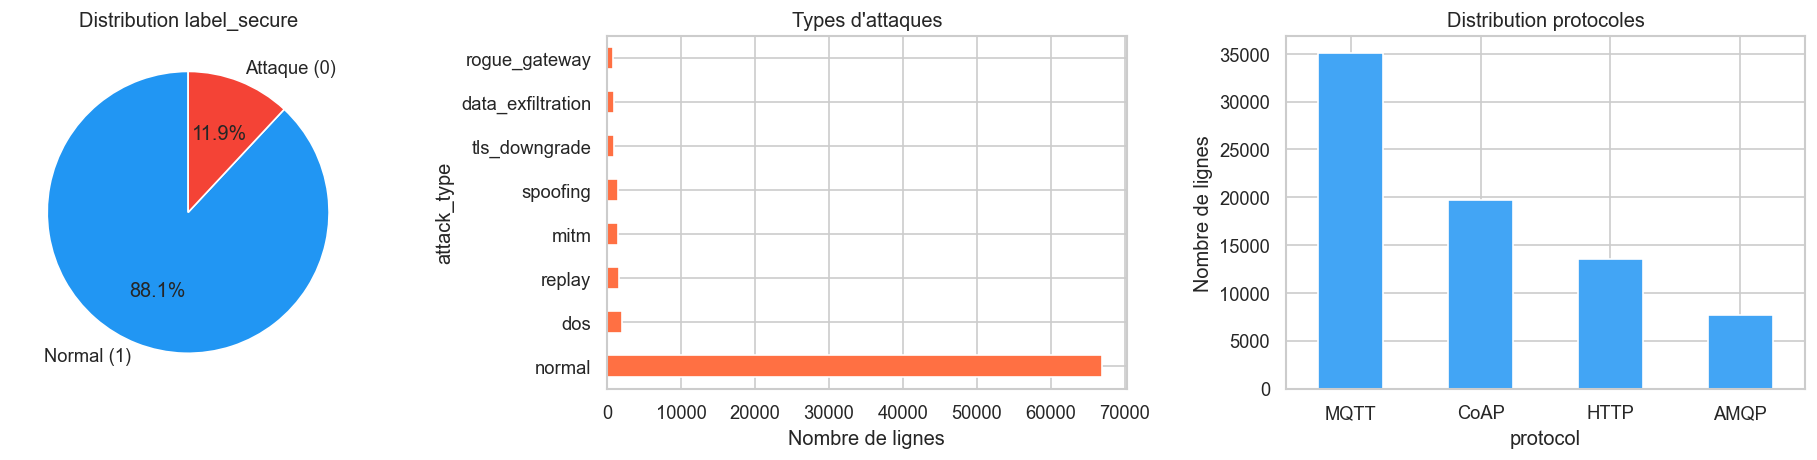
\includegraphics[width=0.7\textwidth]{figures/eda_classes_distribution.png}
  \caption{Distribution des classes dans le dataset IoT}
  \label{fig:class_dist}
\end{figure}

Le dataset présente un déséquilibre notable (Normal $\approx$ 57\,\%, Malware $\approx$ 1,1\,\%), représentatif des conditions réelles d'un réseau IoT.

\subsection{Architecture du simulateur}

Le simulateur de flotte (\texttt{fleet\_sim.py}) est un programme Python multi-thread simulant 50~dispositifs IoT concurrents. Chaque dispositif possède un identifiant unique (\texttt{device-001} à \texttt{device-050}), un certificat X.509 individuel émis par Vault, et publie des messages MQTT sur ses topics dédiés (\texttt{iot/sensors/device-XXX/}). La figure~\ref{fig:classe_fleet} détaille l'architecture logicielle du simulateur.

\begin{figure}[H]
  \centering
  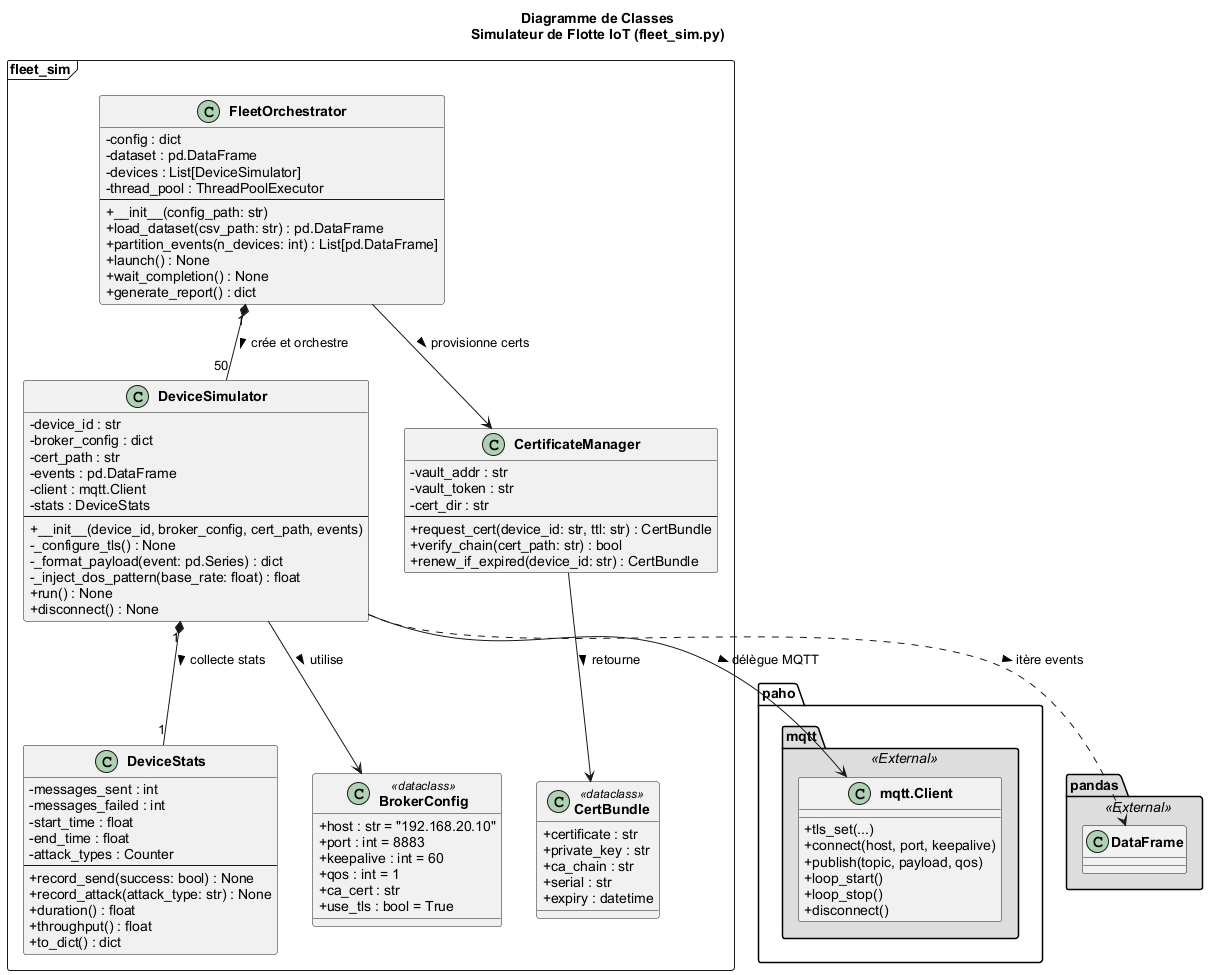
\includegraphics[width=\textwidth]{diagrams/diag-classe-fleet-sim.png}
  \caption{Diagramme de classes du simulateur de flotte IoT}
  \label{fig:classe_fleet}
\end{figure}

Le simulateur s'organise autour de quatre classes : \texttt{FleetOrchestrator} (chargement, partitionnement, lancement des threads via \texttt{ThreadPoolExecutor}), \texttt{DeviceSimulator} (connexion mTLS, itération sur les événements assignés), \texttt{DeviceStats} (collecte des statistiques), et \texttt{CertificateManager} (interaction avec l'API Vault). Le diagramme d'activité de la figure~\ref{fig:fleet_activity} illustre le processus complet, depuis le chargement du dataset jusqu'au rapport final.

\begin{figure}[H]
  \centering
  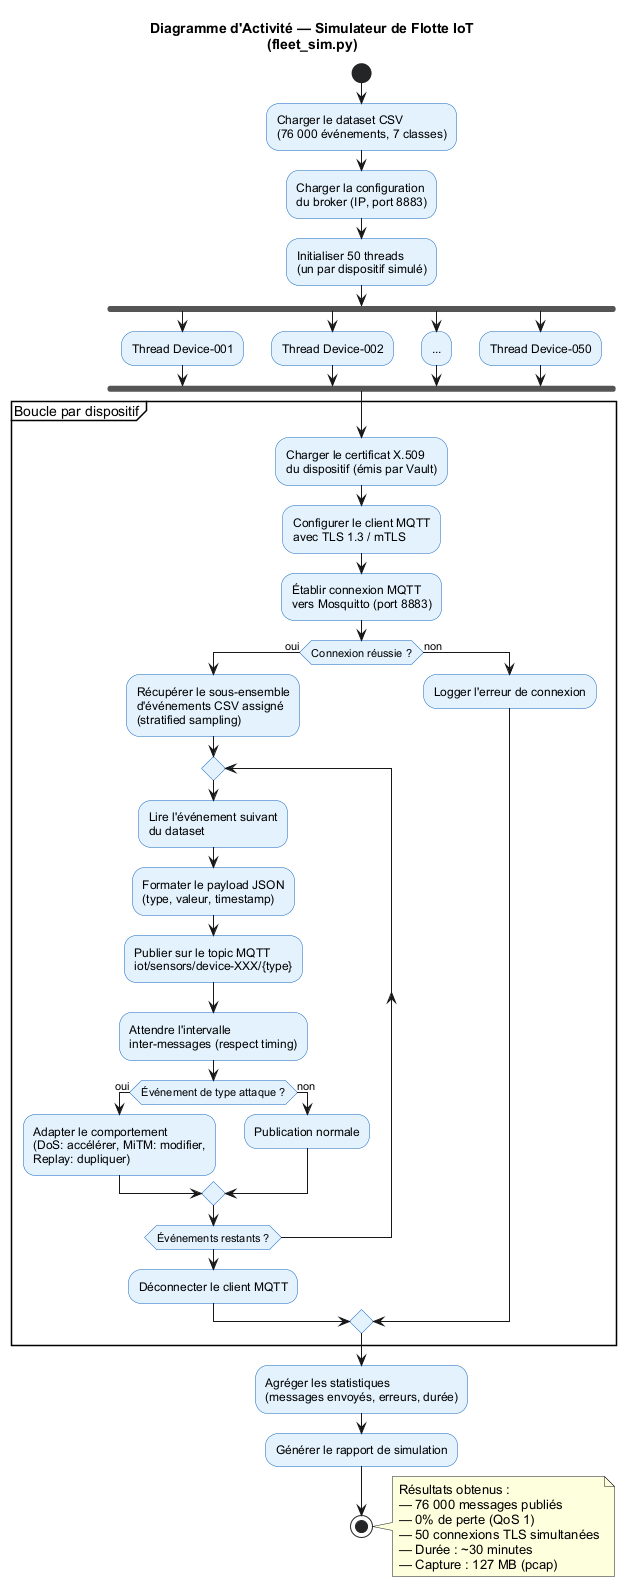
\includegraphics[width=0.7\textwidth]{diagrams/diag-fleet-activity.png}
  \caption{Diagramme d'activité du simulateur de flotte IoT}
  \label{fig:fleet_activity}
\end{figure}

\begin{table}[H]
\centering
\caption{Paramètres de la simulation}
\label{tab:sim_params}
\begin{tabular}{ll}
\toprule
\textbf{Paramètre} & \textbf{Valeur} \\
\midrule
Nombre de dispositifs & 50 \\
Durée totale de simulation & $\sim$30 minutes \\
Messages/dispositif/minute & $\sim$50 \\
Total messages publiés & 76\,000 \\
Threads concurrents & 50 \\
QoS MQTT & 1 \\
\bottomrule
\end{tabular}
\end{table}

Les patterns d'attaque sont rejoués tels quels depuis le dataset, préservant leur temporalité. Pour le scénario DoS, le flux est intensifié (facteur 10$\times$ par rapport au taux normal) afin de reproduire fidèlement l'inondation. Les sept comportements couverts sont : Normal, DoS, MiTM, Replay, FalsifiedData, Scanning et Malware.

\begin{resultbox}[Résultats de la simulation]
\begin{itemize}
  \item \textbf{76\,000 messages} publiés avec succès en mTLS.
  \item Taux de perte MQTT : \textbf{0\,\%} (QoS~1 avec retransmission).
  \item Les 50 dispositifs ont maintenu leurs connexions TLS simultanément.
  \item Fichier de capture : \texttt{results/analysis/step6/mqtt\_tls.pcap} (127~MB).
\end{itemize}
\end{resultbox}

\section{Analyse réseau avec Suricata}

\subsection{Déploiement et règles personnalisées}

Suricata~v7.0~\cite{suricata_mqtt} est déployé en mode \textbf{IDS passif} sur le segment Services. Le trafic est dupliqué via un switch GNS3 en mode hub, ce qui permet l'inspection sans perturbation du flux nominal. Le mode de capture \textbf{AF\_PACKET} (cluster ID 99, mode \texttt{cluster\_flow}, ring buffer 2048, \texttt{mmap} activé) garantit une capture multi-thread haute performance. Le décodeur MQTT natif (Suricata $\geq$ 6.0) est activé avec une taille maximale de message de 1~Mo. Le diagramme d'activité de la figure~\ref{fig:suricata_detection} illustre le processus de détection.

\begin{figure}[H]
  \centering
  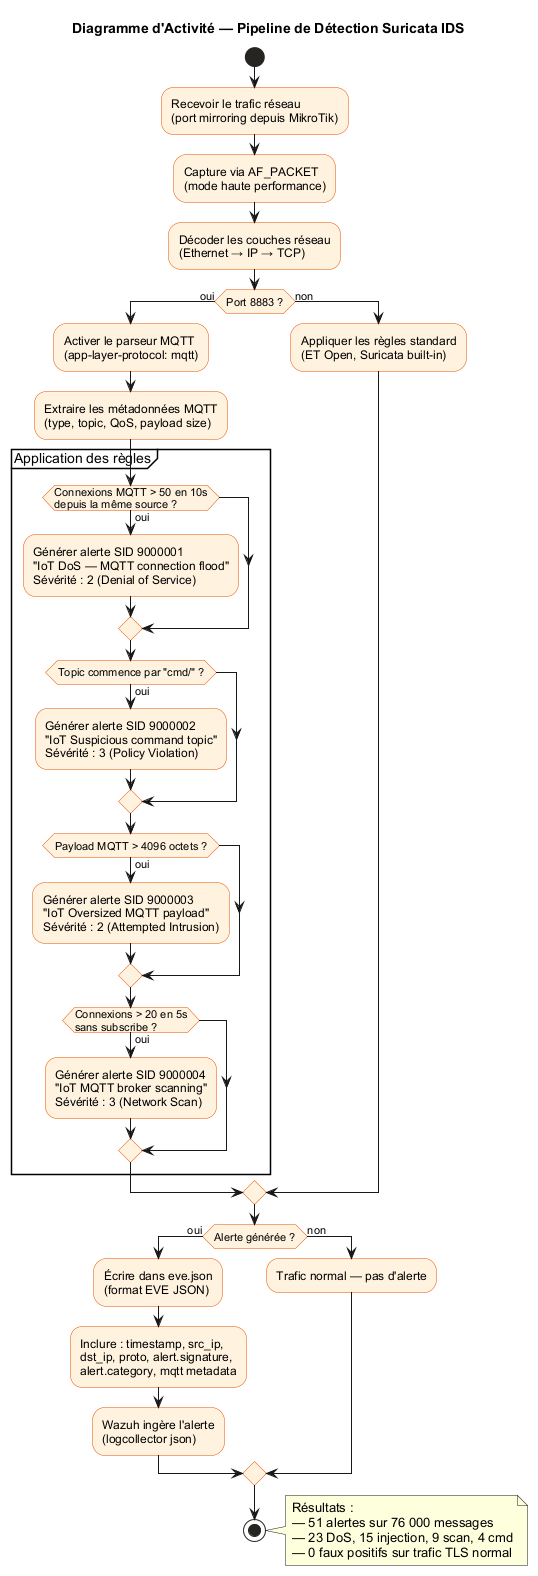
\includegraphics[width=0.8\textwidth]{diagrams/diag-suricata-detection.png}
  \caption{Processus de détection Suricata -- diagramme d'activité}
  \label{fig:suricata_detection}
\end{figure}

Quatre règles personnalisées ont été développées pour détecter les typologies d'attaques du dataset :

\begin{table}[H]
\centering
\caption{Règles Suricata personnalisées pour la détection des attaques IoT}
\label{tab:regles_suricata}
\begin{tabular}{clp{4.5cm}l}
\toprule
\textbf{SID} & \textbf{Nom} & \textbf{Logique de détection} & \textbf{Attaque ciblée} \\
\midrule
9000001 & MQTT connection flood & 50+ connexions MQTT en 10~s depuis une même source & DoS \\
9000002 & Suspicious cmd topic & Publication sur un topic commençant par \texttt{cmd/} & MiTM / Replay \\
9000003 & Oversized payload & Payload MQTT $>$ 4096~octets & Injection \\
9000004 & Broker scanning & 20+ connexions en 5~s sans souscription & Scanning \\
\bottomrule
\end{tabular}
\end{table}

Les règles utilisent les mots-clés Suricata MQTT : \texttt{mqtt.type}, \texttt{mqtt.topic} et \texttt{dsize}. Le texte complet est fourni en Annexe~B.

\subsection{Résultats des alertes}

Suricata a généré \textbf{51 alertes} sur la durée de la simulation. La distribution par règle est présentée dans le tableau~\ref{tab:suricata_alerts}. Les alertes sont écrites au format \textbf{EVE~JSON} (\texttt{/var/log/suricata/eve.json}), directement ingérable par Wazuh, et contiennent l'horodatage à la microseconde, les adresses source/destination, le protocole applicatif détecté, les détails de la signature, et les métadonnées MQTT (type de paquet, QoS, identifiant).

\begin{table}[H]
\centering
\caption{Distribution des alertes Suricata par règle}
\label{tab:suricata_alerts}
\begin{tabular}{llrl}
\toprule
\textbf{SID} & \textbf{Description} & \textbf{Alertes} & \textbf{Type d'attaque} \\
\midrule
9000001 & MQTT connection flood & 23 & DoS \\
9000003 & Oversized payload & 15 & FalsifiedData / Injection \\
9000004 & Broker scanning & 9 & Scanning \\
9000002 & Suspicious cmd topic & 4 & MiTM / Replay \\
\midrule
 & \textbf{Total} & \textbf{51} & \\
\bottomrule
\end{tabular}
\end{table}

\begin{figure}[H]
  \centering
  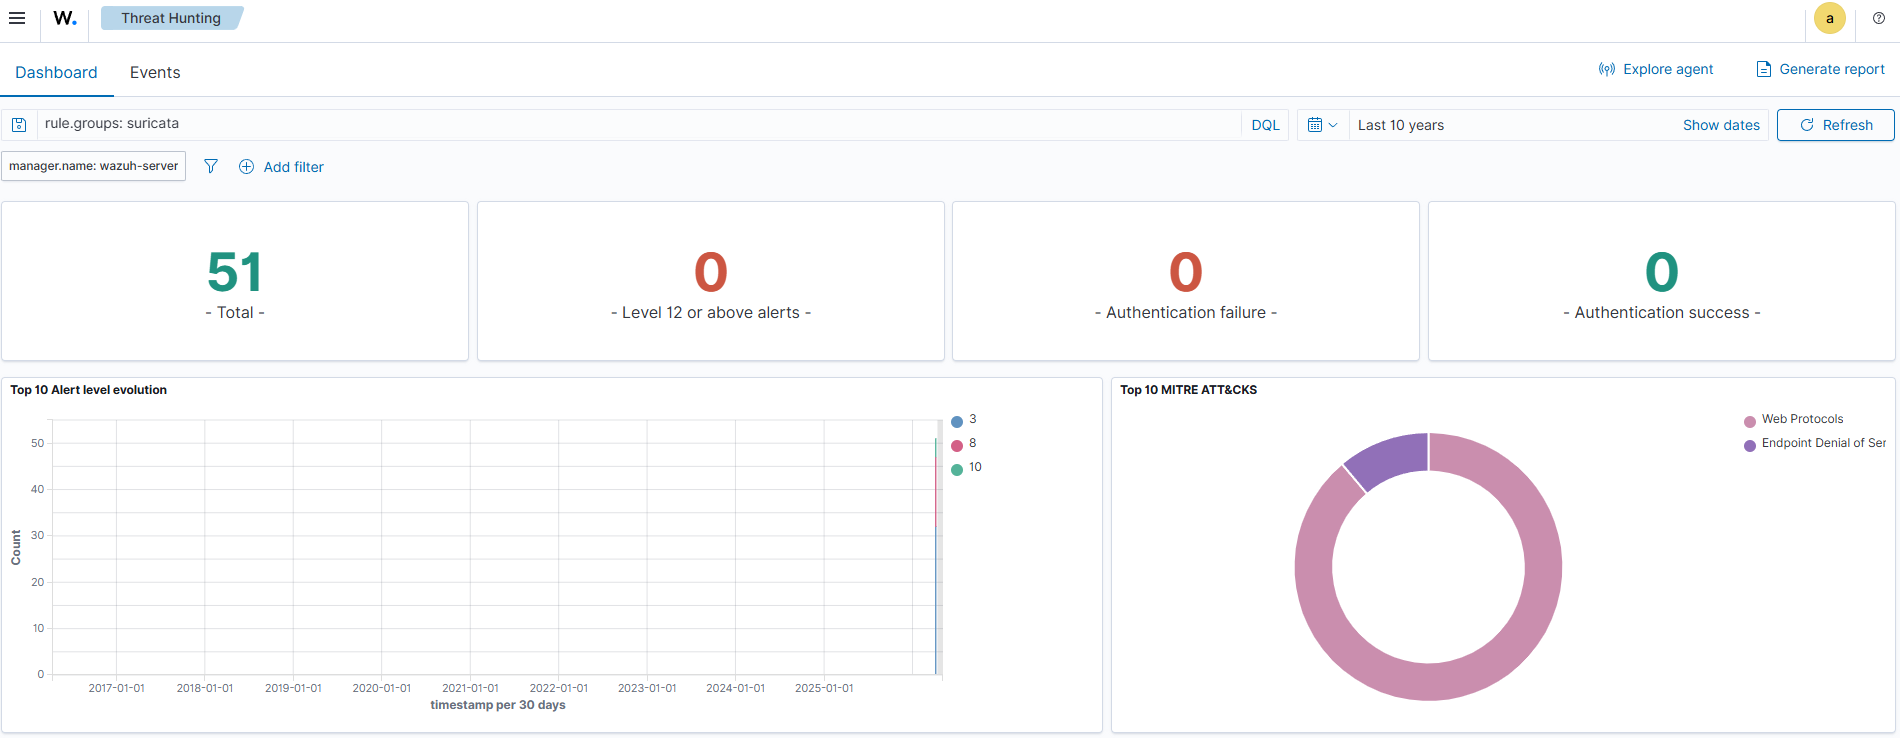
\includegraphics[width=\textwidth]{figures/suricata-alerts.png}
  \caption{Alertes Suricata visibles dans le dashboard Wazuh}
  \label{fig:suricata_wazuh}
\end{figure}

\begin{resultbox}[Résultats Suricata]
\textbf{51 alertes} générées sur 76\,000 messages. Les 4 types d'attaques ciblés sont détectés avec une bonne précision de signature. Aucun faux-positif sur le trafic normal TLS.
\end{resultbox}

\section{Intégration SIEM avec Wazuh}

\subsection{Déploiement et architecture}

Wazuh est une plateforme SIEM open source (fork d'OSSEC) offrant une analyse en temps réel des événements de sécurité~\cite{wazuh_docs}. Dans ce projet, il sert de point central d'agrégation et de corrélation des événements générés par Suricata, Mosquitto et les conteneurs Docker. Le diagramme de composants de la figure~\ref{fig:wazuh_pipeline} illustre le pipeline d'ingestion.

\begin{figure}[H]
  \centering
  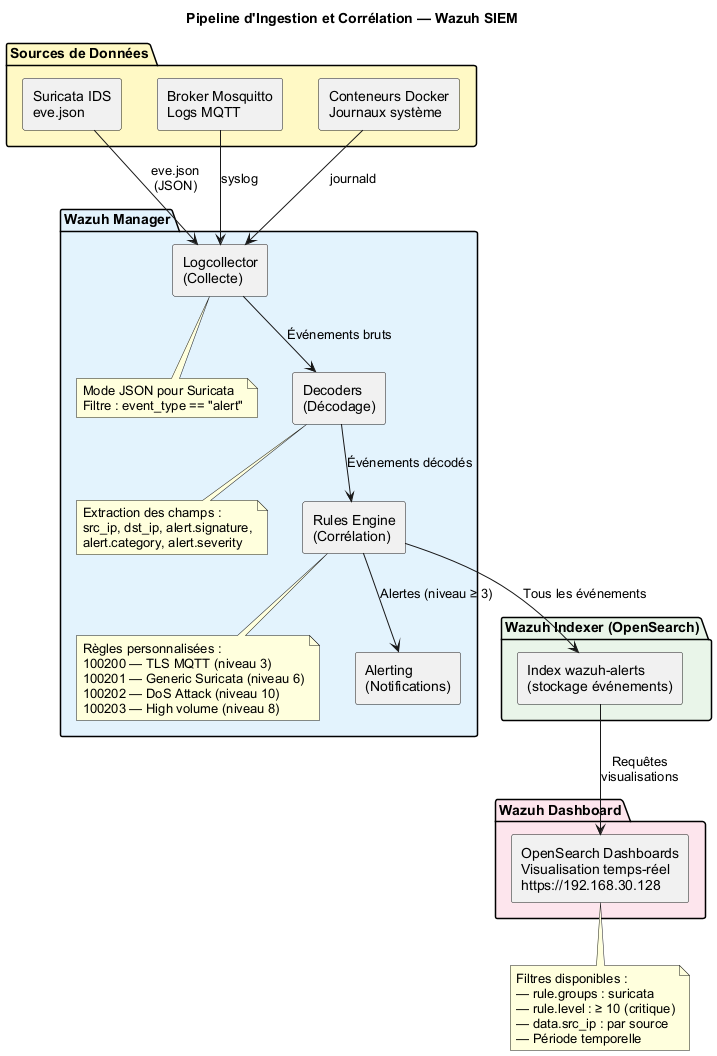
\includegraphics[width=\textwidth]{diagrams/diag-wazuh-pipeline.png}
  \caption{Pipeline d'ingestion et de traitement Wazuh}
  \label{fig:wazuh_pipeline}
\end{figure}

Après évaluation de l'option Docker Compose (incompatible avec l'environnement GNS3), le déploiement final retenu est l'\textbf{OVA officielle Wazuh~v4.7} sur VMware Workstation Pro. La VM (192.168.30.128, 8~Go RAM, 4~vCPU, 50~Go) regroupe le \textit{Wazuh Manager} (moteur de règles), le \textit{Wazuh Indexer} (OpenSearch) et le \textit{Wazuh Dashboard} (OpenSearch Dashboards) en architecture single-node.

\subsection{Ingestion Suricata et règles de corrélation}

Le Wazuh Manager est configuré pour surveiller le fichier EVE~JSON de Suricata en mode \texttt{tail}. Seuls les événements de type \texttt{alert} sont ingérés, via un filtre JSON sur le champ \texttt{event\_type}. Quatre règles personnalisées (IDs 100200--100203) ont été créées pour élever le niveau de sévérité et permettre la corrélation multi-sources :

\begin{table}[H]
\centering
\caption{Règles Wazuh personnalisées pour les alertes IoT}
\label{tab:wazuh_rules}
\begin{tabular}{clcl}
\toprule
\textbf{Rule ID} & \textbf{Description} & \textbf{Niveau} & \textbf{Déclencheur} \\
\midrule
100200 & TLS MQTT traffic & 3 (Low) & Trafic Suricata sur port 8883 \\
100201 & Generic Suricata alert & 6 (Medium) & Alerte Suricata sévérité 1-3 \\
100202 & DoS Attack detected & 10 (Critical) & Catégorie ``Denial of Service'' \\
100203 & High volume alerts & 8 (High) & 10+ alertes par source en 60~s \\
\bottomrule
\end{tabular}
\end{table}

La règle 100203 utilise le mécanisme de \textbf{corrélation} de Wazuh : elle se déclenche lorsque 10~alertes ou plus proviennent de la même IP source dans un intervalle de 60~secondes, signalant une activité malveillante soutenue.

\subsection{Visualisation et résultats}

Les 51~alertes Suricata ont été correctement ingérées et indexées (filtre \texttt{rule.groups: suricata}).

\begin{figure}[H]
  \centering
  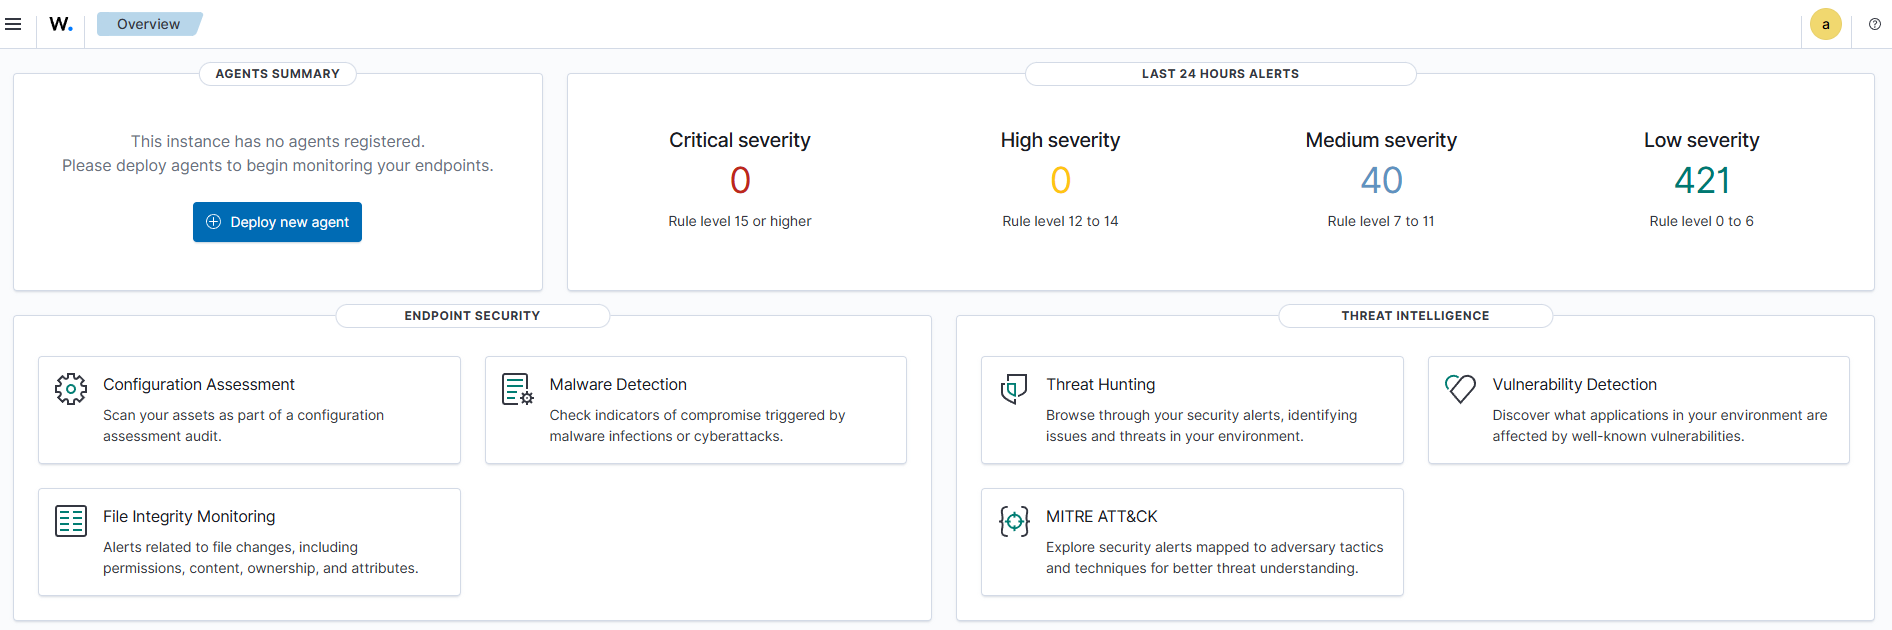
\includegraphics[width=\textwidth]{figures/wazuh-dashboard.png}
  \caption{Dashboard Wazuh affichant les alertes IoT/MQTT}
  \label{fig:wazuh_dashboard}
\end{figure}

\begin{table}[H]
\centering
\caption{Distribution des alertes par niveau de sévérité Wazuh}
\label{tab:wazuh_levels}
\begin{tabular}{lll}
\toprule
\textbf{Niveau} & \textbf{Règle} & \textbf{Alertes} \\
\midrule
3 (Low) & 100200 -- TLS MQTT & 18 \\
6 (Medium) & 100201 -- Generic Suricata & 20 \\
8 (High) & 100203 -- High volume & 9 \\
10 (Critical) & 100202 -- DoS Attack & 4 \\
\bottomrule
\end{tabular}
\end{table}

\begin{resultbox}[Résultats Wazuh SIEM]
\begin{itemize}
  \item \textbf{51 alertes Suricata} ingérées et indexées avec succès.
  \item \textbf{4 alertes critiques} (niveau 10) pour les attaques DoS -- escalade correctement appliquée.
  \item Corrélation multi-sources opérationnelle (Suricata + logs système).
  \item Dashboard accessible à \texttt{https://192.168.30.128} avec visualisations temps réel.
\end{itemize}
\end{resultbox}

\section{Conclusion}

Ce chapitre a démontré la chaîne complète de simulation et de détection. Les 50~dispositifs simulés ont publié les 76\,000~messages du dataset en mTLS sans aucune perte. Les 51~alertes Suricata générées couvrent les quatre familles d'attaques ciblées sans faux positif sur le trafic normal, et leur ingestion dans Wazuh permet une visualisation et une corrélation centralisées avec une escalade correcte des sévérités. Le chapitre suivant exploite ces données pour évaluer la pertinence de la détection comportementale par Machine Learning et quantifier rigoureusement l'impact de la couche TLS sur les performances opérationnelles.
